\chapter{Quantics Fourier Transform}
\label{app:QFT}

The quantics representation of tensors
\cite{Oseledets2009,Khoromskij2011} makes a Fourier transform almost trivial at the tensor-network level.  
For a scalar function \(G(\br)\) represented as a Quantics TT, the Fourier transfor   
\begin{equation}
    \hat{G}(\bk) = \int d \br\; G(\br) e^{i\bk\cdot\br} 
    \label{eq:genericFT}
\end{equation}
results in a very simple MPO-MPO contraction that resembles the operation performed in some quantum computing routines \cite{NielsenChuang2010} (e.g. Quantum Phase Estimation). 

Let us start from the definition of Discrete Fourier Transform (DFT). Consider the variable $G_m = G(x(m))$, discretisation of the one-dimensional function $G(x)$ on a grid with $m=0,\dots,M-1$. The discrete Fourier transform (DFT) of $G_m$ reads 

\begin{equation}
    \hat{G}_k = \sum_{m=0}^{M-1} T_{km}G_m, \quad T_{km} = \frac{1}{\sqrt{M}}e^{-i2\pi k\cdot m/M}
    \label{eq:DFT}
\end{equation}

Represent \(m\) and \(k\) in binary with \(\mR=\log_{2}M\) bits,
\begin{equation}
    m(\bsigma) = \sum_{r=1}^{\mR} \sigma_r 2^{\mR -r }, \quad k(\bsigma') = \sum_{r'=1}^{\mR} \sigma_{r'}2^{\mR-r'}
\end{equation}
so that \(M=2^{\mR}\). Then
\begin{equation}
    T_{\bsigma'\bsigma} = T_{k(\bsigma')x(\bsigma)} = \frac{1}{2^{\mR/2}}\exp \left[ -i2\pi \sum_{rr'} 2^{\mR-r'-r} \sigma'_{r'}\sigma_r \right]
\end{equation}

Re-ordering the bits in “scale–reversed’’ \cite{Fernandez2024,Hiroshi2023} fashion—fusing
\(\sigma'_{\mR-r+1}\), which encodes the scale \(2^{\,r-1}\) in \(k\), with
\(\sigma_{r}\), which encodes the scale \(2^{\mR-r}\) in \(x\)—one can cast
\(T\) as the remarkably low-rank MPO 

\begin{equation}
     \widetilde{T}_{\bsigma'\bsigma} = \raisebox{-7.5mm}{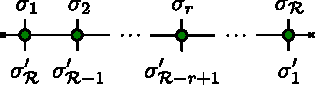
\includegraphics{figures/FTMPO.pdf}}
\end{equation}

whose maximum bond dimension is just \(\chi'=11\) for machine-precision
accuracy \cite{Chen2023}, \(
  \left|
    T_{\bsigma'\bsigma}-\widetilde T_{\bsigma'\bsigma}
  \right|
  \big/
\left|
    \widetilde T_{\bsigma'\bsigma}
  \right|
  \sim\epsilon_{\text{mach}}.
\).

Given a TT of rank \(\chi\), its quantics Fourier transform costs only 
\begin{equation}
  \mathcal O \bigl(\chi^{2}\,\chi'^{2}\,\mR\bigr)
  =\mathcal O \bigl(\chi^{2}\,\chi'^{2}\,\log M\bigr),
\end{equation}
which is exponentially faster than the conventional FFT scaling
\(\mathcal O \bigl(M\log M\bigr)\) \cite{Fernandez2024}.

For a generic \(d\)-variate function \(G(\br)\) the quantics Fourier transform is implemented by applying one 1D QFT per physical dimension. Graphically the operation can be written as  
\begin{equation}
    \raisebox{-2.5cm}{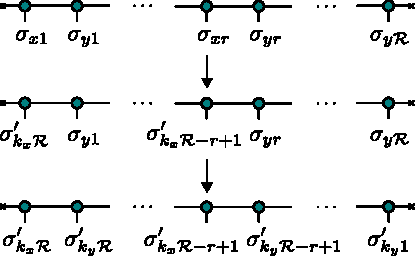
\includegraphics{figures/multiVarFT.pdf}}
\end{equation}
where, in the first step, we act only on the \(x\)-bits with the MPO
\begin{equation}
    \widetilde{T}^{x}_{\bsigma'\bsigma} = \raisebox{-7.5mm}{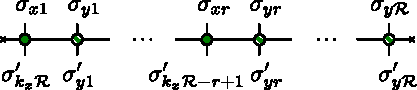
\includegraphics{figures/multiVarFTMPO.pdf}}
\end{equation}

whose non-transforming site tensor factorises as

\begin{equation}
    \raisebox{-7.5mm}{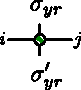
\includegraphics{figures/multiVarFTSiteTensor.pdf}}\;=\;\begin{cases}
        [\mathds{1}]_{i,j} \quad &\text{if}\ \sigma'_{yr} = \sigma_{yr} \\
            [0]_{i,j} \quad &\text{otherwise}.
    \end{cases}
\end{equation}

The construction repeats for the \(y\)- (and \(z\)-, \dots) registers until the full \(d\)-dimensional QFT is obtained. 

\subsection{Rearrangement of quantics meshes}

In the susceptibility calculation of \prettyref{sec:bubbleCalc} we are interested in having the inverse temporal Fourier transform at a shifted Matsubara grid whose centre corresponds to the smallest frequency, namely $\nu_n = \pi\frac{2n + \xi}{\beta}$ with $n= -2^{\mR-1},\dots,2^{\mR-1}-1$. Starting from
\begin{equation}
\begin{aligned}
    G(i\nu_{n'}) &= \beta \int_{0}^{\beta} d\tau  e^{i\nu_{n'}\tau}  G(\tau) = \frac{\beta}{2^{\mR/2}} \sum_{m=0}^{2^\mR-1} e^{i\nu_{n'} \frac{m}{2^\mR}} G_m \\
    &=\frac{\beta}{2^{\mR/2}} \sum_{m=0}^{2^\mR-1} e^{i\pi \frac{(2{n'} + \xi)}{\beta} m}  G_m
\end{aligned}
\end{equation}
and redefining the index \(n=n'-2^{\mR-1}\in[-2^{\mR-1},2^{\mR-1}-1]\) we
obtain 
\begin{equation}
    \begin{aligned}   
    G(i\nu_{n}) = G(i\nu_{n' - 2^{\mR-1}}) &= \frac{\beta}{2^{\mR/2}} \sum_{m=0}^{2^\mR-1} e^{i2\pi\frac{n'm}{2^{\mR}}} e^{i\pi m \frac{\xi - 2^{\mR}}{2^{\mR}}} G_m \\
    &= \beta \sum_{m=0}^{2^\mR-1} T^{(+)}_{n'm} e^{i\pi m \frac{\xi - 2^{\mR}}{2^{\mR}}} G_m
       \end{aligned}
    \label{eq:rearrangedFT}
\end{equation}

with the ``positive'' DFT kernel
\(T^{(+)}_{n'm}=(2^{\mR-1})^{-1/2}e^{+i2\pi n'm/2^{\mR}}\) as defined in \prettyref{eq:DFT}.  
Equation~\eqref{eq:rearrangedFT} shows that the centred Matsubara transform is realised by a standard inverse QFT followed by a diagonal
\emph{phase-rotation} layer \(\mathcal P\) \cite{Hiroshi2023}: 
\begin{equation}
    \beta \text{QFT}^{-1}\mathcal{P}, \qquad 
    \mathcal{P} = \text{U}1(2^{\mR-1}\theta)\cdot\text{U}1(2^{\mR-2}\theta)\cdots\text{U}1(\theta)
\end{equation}
where

\begin{equation}
    \theta=\pi\frac{\xi-2^{\mR}}{2^{\mR}}, \qquad
    \text{U}1(\alpha) = \begin{pmatrix}
        1 & 0 \\
        0 & e^{i\alpha}
    \end{pmatrix}.
\end{equation}

The layer \(\mathcal P\) is an MPO of rank~1, so the extra cost is negligible
compared with the inverse QFT itself.  An analogous modification is applied
to the spatial QFT when, for instance, we would like to center the symmetric Brillouin zone \([-\pi,\pi]^{2}\) on the quantics spatial grid.

These conventions are all employed for the susceptibility calculations reported in \prettyref{sec:bubbleCalc}.